\chapter{Generación del documento de texto}

\section{Diseño}
El documento de texto debe contener toda la información posible de la ontología, organizado en secciones, subsecciones y párrafos. Para alcanzar el documento final, se crearon módulos teniendo como referencia las actividades de la generación de lenguaje natural nombradas en \ref{sec:tareas_gnl}. Los tres módulos principales son emph{macroplanificación}, \emph{microplanificación} y \emph{realización}. Dentro de cada módulo se desarrollaron submódulos, para resolver cada problema específico. 

Si bien en el capítulo anterior se propuso un flujo lineal de información en el organizador de información, en este capítulo, al desarrollar la macroplanificación, se integraron los módulos del organizador de información con los submódulos de la macroplanificación, generando una interacción cíclica entre los módulos. El motivo de esta integración es evitar la creación de interfaces entre los módulos, y el overhead que estas suponen, ya que la creación del árbol de información y la macroplanificación resultan ser procesos equivalentes, por lo que pueden realizarse al mismo tiempo, evitando recorrer el doble de veces la estructura jerárquica. 

En la figura \ref{fig:modulos_plan_documento} se puede ver la integración de los módulos. Los pasos de la interacción entre los módulos se encuentran enumerados en orden, siendo los pasos 5 y 6 repetibles hasta que no hayan más grupos de entidades (correspondientes a niveles en la jerarquía de la estructura).

\begin{figure}[H]
    \centering
    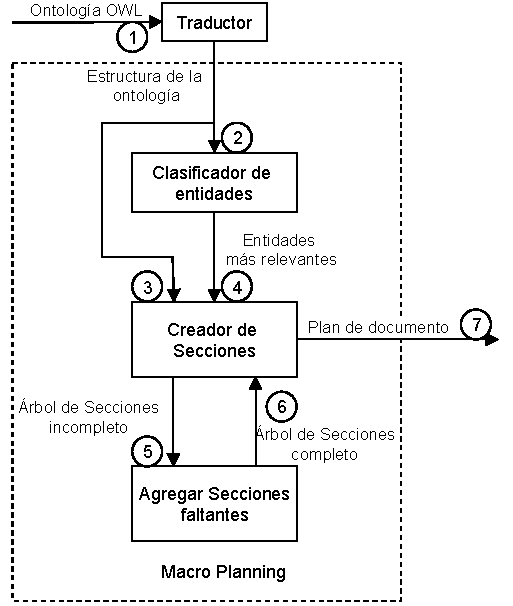
\includegraphics[width=12cm, height=5cm]{img/generacion_documento/modulos_plan_documento.pdf}
    \caption{Integración de módulos para la generación del plan de documento.}
    \label{fig:modulos_plan_documento}
\end{figure}

Cabe aclarar que, si bien la estructuración del documento se determina con base en el árbol de entidades, en el documento final la realización de la estructura (secciones y párrafos) se retrasa hasta tener mayor información acerca de su contenido, es decir, luego de la etapa de microplanificación. Estas tareas se encuentran desarrolladas en los módulos de microplanificación y realización, los cuales se muestran en la figura \ref{fig:modulos_documento_final}.

\begin{figure}[H]
    \centering
    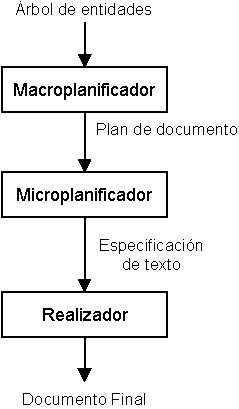
\includegraphics[width=12cm]{img/generacion_documento/modulos_documento_final.pdf}
    \caption{Módulos para la generación del documento final.}
    \label{fig:modulos_documento_final}
\end{figure}

\section{Diseño macro planning}
En esta tarea se planificará la estructura del documento. Como nombramos anteriormente, la organización a priori de la información, realizada en el capítulo anterior, facilita la tarea de macro planificación. Por este motivo, se decidió hacer una arquitectura monolítica entre el organizador de información y el macroplanificador. Sin embargo, para evitar seguir trabajando con árboles de entidades, se construyó un conjunto de componentes para comenzar con el documento de texto. De esta manera, el plan de documento, representado en la figura \ref{fig:modulos_plan_documento} con el número 9, se corresponde a un conjunto de clases que definen una representación interna de un documento de texto. 

Esta representación prepara el terreno para que, luego de la microplanificación, el realizador decida el diseño final del documento.

La creación de la representación interna del documento de texto tiene en cuenta los siguientes criterios:
\begin{itemize}
    \item A cada clase le corresponde una sección.
    \item Cada sección está compuesta de al menos un párrafo y un título.
    \item Cada párrafo trata un único tópico, el cual puede ser una clase o un individuo. También, un párrafo puede o no tener alguna sentencia. Este criterio se debe a que no todas las entidades tienen asociados axiomas que la describan.
    \item Las \emph{owl:ObjectProperties} solo pueden ser tópico de una sección cuando se utilizan para agrupar información de una clase. Cuando una 
\end{itemize}

\subsection{Diagrama de clases}
En la figura \ref{fig:diagrama_clases_macroplanificador} se muestra el diagrama de clases correspondiente al macroplanificador. El componente principal que integra el macroplanificador con el organizador de información es la clase TextManager. Esta clase se encarga de crear la clase Text, que es la representación interna de un documento de texto. El documento está compuesto por Secciones, Párrafos y Sentencias. Cada sentencia tiene como información a su tópico y lo que se dice de su tópico, en forma de entidades OWL.

\begin{figure}[H]
    \centering
    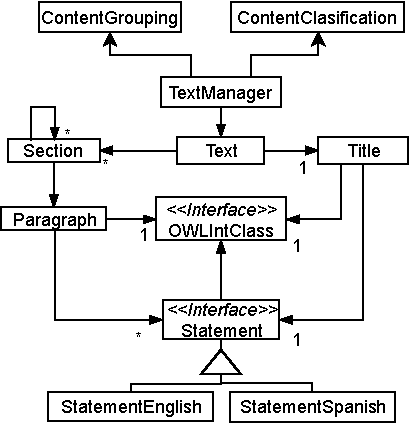
\includegraphics[width=10cm, height=7cm]{img/generacion_documento/diagrama_clases_macroplanificador.pdf}
    \caption{Diagrama de clases del generador del documento de texto.}
    \label{fig:diagrama_clases_macroplanificador}
\end{figure}

\section{Implementación macro panning}

\section{Diseño micro planning}
%El objetivo de esta etapa es organizar el contenido de cada axioma para crear una sentencia gramaticalmente aceptable.

Como ya organizamos y planificamos el documento, ahora debemos centraremos en describir en lenguaje natural a una entidad, a partir de los axiomas que la describen en la ontología. Esta descripción en lenguaje natural se alcanza a través de uno o varias oraciones producidas con una estructura que se adapte a la gramática del lenguaje español.

Como existen diversas estructuras sintácticas para expresar un mismo contenido, a modo de simplificación se asoció a cada constructor OWL solo algunas formas de verbalización. Se trató de generar oraciones que sean fieles al significado expresado en los axiomas y de evitar ambigüedades.

\subsection{Tipos de oraciones}
Teniendo en cuenta la naturaleza jerárquica de las construcciones OWL, se puede verbalizar un axioma considerando dos tipos de oraciones, las compuestas y las complejas. Sabiendo qué información contiene cada uno de los axiomas (\emph{equivalentClass, disjointWith, subClass, superClass, domain y range}), se pueden unir las oraciones, generando oraciones compuestas, a través de una relación de coordinación o yuxtaposición.

En un nivel de mayor granularidad, se tienen las restricciones (\emph{cardinalidad, complemento, unión, intersección}, etc.) con las cuales es posible generar oraciones complejas, subordinando las expresiones que se encuentran anidadas.

\subsection{Flujo de información y sintaxis del texto}
Como la oración se compone de varios niveles jerárquicos de relaciones entre entidades OWL, hay que determinar cómo es el flujo de información durante la exploración jerárquica y qué información requiere cada constructor para poder componer una oración gramaticalmente aceptable. 

%Algunos operadores, como la intersección, requieren información anterior y posterior para tomar una decisión adecuada, por lo que el flujo de información debe hacerse en ambos sentidos durante el análisis del grafo de la ontología: top-down y bottom-up. 
%Una forma de resolver este problema, es recorrer recursivamente desde la raíz enviando información hacia las hojas, y al llegar a una hoja comenzar a crear las partes de la oración, componiendo una oración desde atrás hacia adelante. De esta manera, en la secuencia de invocación a la llamada recursiva se puede heredar información, y durante el retorno de la llamada recursiva se puede sintetizar información acerca de cómo se está componiendo la oración, y se puede tener conocimiento de qué se está diciendo para tomar mejores decisiones gramaticales.
%Al momento de decidir cómo verbalizar un operador, se requiere saber qué  operador es el ancestro inmediato, por lo que la información heredara debe contener al menos al operador que está en el nivel superior inmediato. 
El enfoque adoptado para crear la sintaxis de las oraciones se basa en un recorrido bottom-up de la jerarquía de un axioma, sintetizando la información reunida en cada constructor. Además, la oración comienza a construirse desde atrás hacia adelante, es decir que la oración se va componiendo de derecha a izquierda a medida que se sube en los niveles de la jerarquía.

La principal información requerida en los niveles superiores es qué función cumple la oración parcialmente formada en los niveles inferiores, por lo que la información sintetizada debe estar compuesta al menos del tipo de componente oracional que genera cada operador. Los componentes que retorna cada operador se definen a continuación:
\begin{itemize}
    \item Clase: término (T).
    \item Propiedad: sintagma verbal (SV).
    \item Operadores de cuantificación: SV.
    \item Unión: oración disyuntiva (union).
    \item Intersección: oración copulativa u oración subordinada, que en ambos casos retorna el tipo intersection.%oración copulativa (OC), oración subordinada (OS) u oración copulativa negativa (OCN).
    \item Operadores con cardinalidad: SV.
    \item Complemento: oración negativa (ON).
\end{itemize}

Estos componentes de una oración no intentan ser exhaustivos ni completamente fieles a la sintaxis del español, sino que intentan acaparar de la forma más general los posibles resultados de cada operador, para mantener una sintaxis sencilla y aceptable. Una clase, por ejemplo, podría cumplir la función de sintagma nominal, adjetival o adverbial, pero para simplificar la nomenclatura, se retorna un tipo más genérico y al momento de usar una clase, de ser necesario, se resuelve la composición en función de los elementos que la constituyen. Como veremos más adelante, a veces es innecesario discriminar los tipos de sintagmas.

\subsection{Tareas del microplanning}
Separaremos las tareas de microplanning en tres tareas principales: la verbalización de los constructores OWL, en la eliminación de información redundante entre oraciones, y el reemplazo de entidades nombradas por expresiones de referencia.


\subsubsection{Consideraciones previas}
\noindent {\bf Convención y suposiciones del nombrado de entidades} \\
Para no limitar la aplicación a una convención de nombrado, no se requiere una forma estricta para nombrar las entidades en una ontología. Sin embargo, nos basamos en algunas suposiciones que resultan natural al crear una ontología:
\begin{enumerate}
    \item Las entidades pueden tener su nombre ya sea en la IRI o en un label\footnote{Estas opciones son excluyentes, al verbalizar una ontología solo se extraen los nombres de un solo lugar, por lo que todos los nombres deben ser extraídos de IRI o de label sin combinarse}. Si el nombre es extraído de una IRI, debe estar escrito con el estilo CamelCase. Si el nombre se extrae de un label, debe estar escrito en lenguaje natural, y debe tener el idioma del label (en este caso, español ``es'' o ingles ``en'').
    \item No hay condiciones para el nombre de una clase, sin embargo es preferible que contenga al menos un sustantivo.
    \item No hay condiciones para el nombre de una propiedad, sin embargo es preferible que contenga al menos un verbo. 
    
    No se reconocen verbos implícitos, por lo que si se quiere expresar, por ejemplo, que una clase \emph{está localizada en} algún lugar, la propiedad debería llamarse \emph{estáLocalizadaEn} y no \emph{localizadaEn}. Al igual que los verbos, no es conveniente omitir las preposiciones finales, por ejemplo, en la propiedad \emph{esParte}, es recomendable utilizar \emph{esParteDe}.
\end{enumerate}

Estas condiciones ayudan a mejorar la fluidez del texto y no suponen una gran carga en los desarrolladores de ontologías.
\\

\noindent {\bf Tratamiento sintáctico de los nombres de entidades}\\
Para facilitar el entendimiento de las secciones referidas al micro planning, se explicará cómo fueron tratados los nombres de las entidades, desde el punto de vista sintáctico. 

Dado que los nombres de las entidades pueden no corresponderse fielmente con la gramática de un lenguaje (por falta de palabras funcionales, tales como artículos o preposiciones), se optó por no realizar un análisis sintáctico a los nombres. Se consideró, a cada conjunto de palabras que conforman el nombre de una entidad, como un componente incompleto que es parte de una oración más grande. Por este motivo, se divide en dos partes fundamentales: una parte inicial y un complemento, entre los cuales pueden insertarse nexos y cuantificaciones. A continuación se explican cómo se reconocen ambas partes en las clases y propiedades:
\begin{itemize}
    \item Los nombres de las propiedades (en los que suponemos existe al menos un verbo), se considera como parte inicial a todas las palabras desde el inicio hasta el primer verbo, incluído el verbo. El complemento se conforma con todas las palabras que siguen al verbo. Por ejemplo: la propiedad \emph{tiene color} se compone de parte inicial: \emph{tiene}, y complemento: \emph{color}. La propiedad \emph{se solapa con} se compone de \emph{se solapa} como parte de inicial, y \emph{con} como complemento.
    \item Los nombres de las clases (en los que suponemos existe al menos un sustantivo), se considera como parte inicial a todas las palabras desde el inicio hasta el primer sustantivo, incluido el sustantivo. El complemento se conforma con todas las palabras que siguen al sustantivo. Por ejemplo: la clase \emph{agente social}, tiene como parte inicial \emph{agente} y complemento \emph{social}. La clase \emph{cobertura de pizza} se compone de \emph{cobertura} con complemento \emph{de pizza}.
    \item Los nombres de los individuos son tratados igual que los nombres de las clases.
\end{itemize}


\subsubsection{Verbalización de constructores OWL}
Esta tarea se encarga de componer las oraciones según la información de cada constructor OWL. Las oraciones pueden enfocarse ya sea en una \emph{owl:Class} o  \emph{owl:NamedIndividual}. Cuando se enfocan en una \emph{owl:Class}, pueden contener la siguiente información: clases equivalentes, disjuntas, subclases, superclases, sus instancias y las propiedades en las que participa. Cuando se enfoca en un \emph{owl:NamedIndividual}, puede contener información acerca de los valores de sus propiedades.

Para cada uno de estos tipos de información, se pueden presentar una o varias oraciones. Las oraciones que tratan el mismo tipo de información se organizan adyacentemente entre ellas.
\\

En algunos constructores, tener un único patrón gramatical resulta insuficiente, debido a que pueden recibir distintas estructuras gramaticales como entrada, que requieren diferentes formas de componerse. Por lo tanto, se diseñó más de una forma de componer la información en algunos constructores, mejorando la fluidez e interpretación de las oraciones. 

Para reconocer cómo componer las oraciones en cada constructor, se revisó empíricamente los axiomas de algunas ontologías, y se buscó utilizar oraciones que sean lo más genéricas posibles, que permitan la comprensión de los axiomas, sin requerir una definición exhaustiva de todas las posibles composiciones. 

Se tienen en cuenta los siguientes descriptores de clases: cardinalidad, complemento, unión, intersección y cuantificación. A continuación se explican los patrones gramaticales usados para cada constructor. El signo $+$ corresponde a la concatenación de cadenas.
\\

{\bf Restricción de cardinalidad \emph{ObjectCardinalityRestriction}}
\begin{itemize}
    \item ``parte inicial de la propiedad + complemento de la propiedad + enlace + cardinalidad + clases sobre las que se aplica la restricción''.

    \item ``parte inicial de la propiedad + enlace + cardinalidad + complemento de la propiedad''

    \item ``parte inicial de la propiedad + enlace + cardinalidad + clases sobre las que se aplica la restricción''
\end{itemize}

En los casos donde sea posible, si la clase sobre la que se aplica la restricción es \emph{owl:Thing}, se reemplaza por el rango de la propiedad, el complemento de la propiedad o por último por la palabra ``cosa''.

El enlace hace referencia a los siguientes enlaces: \emph{como mínimo}, \emph{como máximo} y \emph{exactamente}, dependiendo del operador \emph{MinCardinality}, \emph{MaxCardinality} y \emph{ExactCardinality} respectivamente.

Ejemplo: para la clase ``pizza interesante'', se tiene el axioma: ``tieneCobertura min 3 owl:Thing'', que puede verbalizarse como ``tiene como mínimo 3 coberturas de pizza''. La parte de la oración que se corresponde a \emph{coberturas de pizza}, es extraída del rango de la propiedad.
\\

{\bf Restricción de cardinalidad \emph{DataCardinalityRestriction}}

\begin{itemize}
    \item ``parte inicial de la propiedad + enlace + cardinalidad + complemento de la propiedad''.

    \item ``parte inicial de la propiedad + enlace + cardinalidad + complemento de la propiedad''

    \item ````tiene'' + enlace + cardinalidad + nombre completo de la propiedad'' (en caso de que no tenga verbo)
\end{itemize}

Los enlaces elegidos son: \emph{al menos}, \emph{como máximo} y \emph{exactamente}, dependiendo del operador \emph{MinCardinality}, \emph{MaxCardinality} y \emph{ExactCardinality} respectivamente.
\\

{\bf Restricción de cuantificación \emph{QuantifiedObjectRestriction}}
\begin{itemize}
    \item ``verbo de la propiedad + ``como'' + complemento de la propiedad + enlace + clases sobre las que se aplica la restricción''
    \item ``verbo de la propiedad + enlace + clases sobre las que se aplica la restricción''
    \item ``verbo de la propiedad + enlace + ``a'' + clases sobre las que se aplica la restricción''
    \item ``verbo de la propiedad + ``a'' + enlace + clases sobre las que se aplica la restricción''
    \item ``verbo de la propiedad + complemento de la propiedad + enlace + clases sobre las que se aplica la restricción''
    \item ``verbo de la propiedad + enlace + ``algunos/algunas de los/las siguientes:''+ clases sobre las que se aplica la restricción''
\end{itemize}
Los enlaces elegidos son: \emph{algún/alguna/algo} para el cuantificador existencial y \emph{exclusivamente} para el cuantificador universal.

Ejemplo: la clase ``Margherita'' que es subclase de ``PizzaConNombre'', tiene el axioma ``tieneCobertura only 
    (CoberturaDeMozzarella or CoberturaDeTomate)'' (siendo only el cuantificador universal), el cual se traduce a ``tiene cobertura de mozzarella o tomate''. También posee dos axiomas equivalentes al anterior: ``tieneCobertura some CoberturaDeMozzarella'' y ``tieneCobertura some CoberturaDeTomate'', (siendo some el cuantificador existencial), los cuales se traducen a ``tiene alguna cobertura de mozzarella'' y ``tiene alguna cobertura de tomate''.
\\

{\bf Restricción de cuantificación \emph{QuantifiedDataRestriction}}
\begin{itemize}
    \item ``verbo de la propiedad + enlace + complemento de la propiedad + ``de tipo'' + rango''
    \item ``verbo de la propiedad + complemento de la propiedad + enlace + ``de tipo'' + rango''
\end{itemize}
Los enlaces elegidos son: \emph{algún/alguna/algo} para el cuantificador existencial y \emph{exclusivamente} para el cuantificador universal.
\\

{\bf Restricción N-Ary \emph{UnionOf}} 
\\
Como representa una secuencia de elementos, en la que uno o más elementos pueden ser verdaderos, se eligió concatenar a todos los elementos con el conector disyuntivo ``o''. Sean e1, e2,...,eN los elementos de la unión, el patrón gramatical elegido es: ``e1, e2, ..., eN-1 \emph{o} eN''.
\\

{\bf Restricción N-Ary \emph{InterseccionOf}} \\
La intersección da lugar tanto a la adición como a la subordinación de oraciones. Antes de verbalizar una intersección, se ordenan sus componentes de mayor a menor prioridad, teniendo en cuenta que: T, ON, union, intersection tienen la misma prioridad, y SV tiene menor prioridad. 

Para determinar cómo verbalizar una intersección, se tienen en cuenta las siguientes condiciones:
\begin{itemize}
    \item Si la intersección tiene dos operandos:
        \begin{itemize}
            \item Si el primero es de tipo T  y el segundo SV, se subordina la segunda oración de la siguiente manera:
            ``contenido primer operando + ``que'' + contenido segundo operando''
            \item en cualquier otro caso, se coordinan los operandos:
            ``contenido primer operando + ``y'' + contenido segundo operando''
        \end{itemize}
        \item Si la intersección tiene más de dos operandos, se agrupan según el tipo  (T, SV, ON) y luego se coordinan con la conjunción ``y''.
        
\end{itemize}

Ejemplo, el axioma de clase equivalente ``Pizza and (tieneCobertura some (CoberturaDePizza and (tienePicante some MuyPicante)))'' de la clase pizzaPicanteEquivalente, contiene dos intersecciones las cuales poseen los mismos componentes: T$+$SV, por lo que utilizamos el conector \emph{que} para subordinar el segundo operando. Con este criterio, el axioma anterior sería ``pizza picante es una pizza \emph{que} tiene alguna cobertura de pizza \emph{que} tiene algún picante muy picante''.

En caso de asociar la intersección al conector \emph{y} sin tener en cuenta el contexto, se generaría una oración como la siguiente ``pizza picante es una pizza \emph{y} tiene alguna cobertura de pizza \emph{y} tiene algo muy picante'', dando lugar a ambigüedad, pues la segunda ``y'' podría cumplir la función de adición, interpretándose que la pizza tiene algo picante, en lugar de cumplir una función de subordinación, donde la interpretación correcta es que la cobertura de la pizza es picante. 
        %\item OWLObjectOneOf sirve para la enumeración de los individuos, por lo que se toma el mismo criterio que en la Unión para verbalizarlo.
        %\item OWLObjectComplementOf ...
        %\item OWLObjectHasSelf ..
        %\item OWLObjectHasValue ..
        %\item OWLObjectInverseOf ..


%no es informacion estrictamente redundante.
%\subsubsection{Eliminación de información redundante}
%En ocasiones la verbalización de axiomas diferentes presentan la misma información, lo que vuelve al texto redundante. Para evitar la redundancia, se eliminan las sentencias que contengan información en común entre los distintos tipos de relaciones owl. Por ejemplo: en la ontología wine se listan las propiedades que tienen como dominio wine ``wine has body, has sugar, etc...'' pero también se listan las superclases anónimas, por ejemplo el siguiente axioma: ''wine hasBody exactly 1 owl:Thing'', lo que se traduce en ``wine has one body''. Luego de verbalizar las propiedades y las superclases anónimas, se tienen oraciones como ``wine has body'' y ``wine has one body'', por lo que se puede omitir la primera que es menos específica. Como criterio, se verbalizan las superclases anónimas y luego las propiedades que no fueron usadas se agregan para complementar la información.

\subsubsection{Expresiones de referencia}
Teniendo en cuenta que cada párrafo trata centralmente un único tópico, el conjunto de oraciones perteneciente a ese párrafo hacen referencia a una única entidad. Esto facilita la referenciación, dado que al no intercalar tópicos como focos de atención se reduce la posibilidad de ambigüedad.

Para dar lugar a las expresiones de referencia, se hereda un atributo con el nombre de la clase descrita en el párrafo durante el recorrido jerárquico de cada axioma, para poder usarla o reemplzarla por la expresión adecuada. %Sin embargo, no es muy común (y por lo tanto no es tan necesario) crear expresiones de referencia dentro de la verbalización de los axiomas, ya que por lo general no son largas explicaciones, y no se cambia el tópico principal durante la composición de las sentencias. 
%Por el contrario, cuando se tratan diferentes axiomas acerca de un mismo tópico, existen momentos en los que resulta adecuado utilizar una expresión de referencia, para retomar con énfasis el tema principal.
Además de la posibilidad de referenciar una entidad durante el recorrido jerárquico dentro de un axioma, también se requiere la referenciación entre axiomas, lo que resulta trivial, al estar agrupados bajo un mismo párrafo. 

Para llevar a cabo la referenciación, se tuvo en cuenta el uso de pronombres demostrativos, a veces, acompañados por el primer sustantivo (si posee) del nombre de la entidad.

%Otro tipo de referencias, se da en el momento de explicar una clase. Cuando se crea una sección hablando acerca de una clase \emph{A}, esa sección no vuelve a crearse si existe una clase \emph{B} cuya descripción requiere que se explique la clase \emph{A}, sino que en la clase \emph{B} se hace referencia a la sección donde ya fue explicada la clase \emph{A}. Esto permite reutilizar las secciones y evita agregar información redundante en el texto.

\subsubsection{Agregación de sentencias}
La agregación de sentencias ocurre en dos lugares. Uno es durante el proceso de producción de una oración en el constructor NAry; el otro es durante el proceso de creación de párrafos, es decir, agregación inter-oraciones.

%de marco metodologico para la gnl
Basaremos la agregación en la conjunción por componentes compartidos. El objetivo es que los elementos en común aparezcan una sola vez, mediante elipsis del componente repetido, por ejemplo:
\begin{itemize}
    \item Sean las oraciones: \emph{la casa tiene color rojo}, \emph{la casa tiene color azul} y \emph{la casa tiene color verde}, al comparar linealmente las oraciones, se elimina de las consecutivas oraciones la parte inicial que tengan en común. El resultado de esta agregación es: \emph{la casa tiene color rojo, azul y verde}.
\end{itemize}
    
\begin{itemize}
    \item {\bf Agregación en constructor NAry}: en las situaciones en las que este constructor se utiliza para enumerar sentencias, como el orden de los elementos enumerados no altera el significado de la oración, se optó por agrupar los elementos según su función (T, SV, ON). Para el grupo de sentencias T, se omitió información inicial de la sentencia, que se corresponda léxicamente con el complemento del tópico al que describen. 
    
    Para los grupos SV y ON, se ordenaron por verbo, y cada verbo aparece una sola vez, acompañado por la enumeración de los complementos de cada elemento. Para mejorar más la calidad del texto, también se omitieron las partes iniciales de los complementos que coinciden léxicamente.
    
    \item {\bf Agregación entre sentencias}: esta agregación se aplica cuando se recorren las sentencias para armar un párrafo. Además de agrupar las sentencias por función, también se separan por constructor, obteniendo así 7 grupos: \emph{ObjectSomeValuesFrom, ObjectAllValuesFrom, intersection, union, ObjectHasValue, T, ON y SV}. De esta manera, para cada grupo, se realiza la agregación, de manera independiente entre ellos.
\end{itemize}

\subsection{Diagrama de clases}
En la figura \ref{fig:diagrama_clases_microplanificador} se puede ver el diagrama de clases asociado al módulo de micro planificación. Las subclases de \emph{OWLRestriction} tienen la capacidad de generar las oraciones, según el tipo de restricción que represente.

\begin{figure}[H]
    \centering
    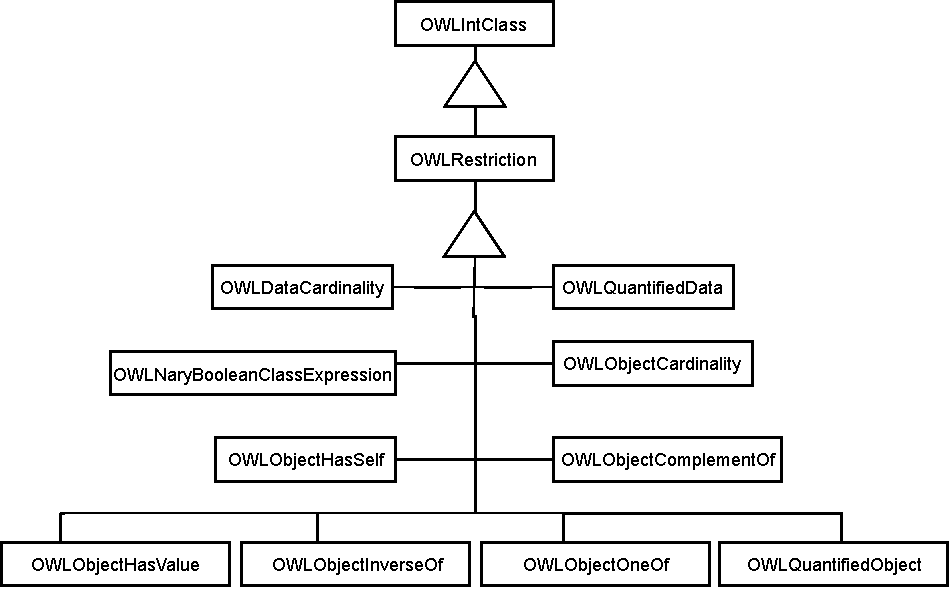
\includegraphics[width=10cm, height=7cm]{img/generacion_documento/diagrama_clases_microplanificador.pdf}
    \caption{Diagrama de clases del micro planificador.}
    \label{fig:diagrama_clases_microplanificador}
\end{figure}


\section{Implementación micro panning}

\subsection{Recursos usados}

\section{Diseño del realizador}
Este módulo se encarga de la tarea de diseñar la estructura final del documento, definiendo criterios para decidir si la información organizada se corresponde a secciones o párrafos.

Para simplificar el documento de salida, solo se consideraron dos niveles de información en el documento: el nivel más alto se corresponde a las secciones (o capítulos) y sub-secciones, y el nivel más bajo a los párrafos. 

Para llevar a cabo esta planificación, se buscó medir la información a verbalizar, por lo que se propuso como métrica principal a la cantidad de sentencias presentes en la descripción de un tópico. Este es el único parámetro para reconocer si a un tópico le corresponde una estructuración asociada a una sección o un párrafo. 

\subsection{Secciones y párrafos}
Una sección agrupa uno o más párrafos o sub-secciones, por lo que en una sección puede existir más de un tópico, con la condición de que esos tópicos tengan una relación, ya sea de hermanos o de hijos. Estas relaciones se obtienen de la estructura en árbol resultado de la macroplanificación. 

Para decidir si un tópico es planificado como una sección, se utiliza como medida la cantidad de sentencias que posee y si tiene algún tópico que a su vez deba ser planificado como una sub-sección.

El valor mínimo de sentencias usado para decidir si se planifica como una sección es de cinco sentencias. Para agregar flexibilidad, el algoritmo queda parametrizado con esta unidad de medida, por lo que puede personalizarse para variar la granularidad del texto de salida, forzando a crear secciones con diferentes cantidad de sentencias, lo que permite variar el diseño del documento de salida.

Otro criterio usado en complemento de la cantidad de sentencias, es si para un tópico existe algún sub-tópico que requiera planificarse como sección, permitiendo anidar secciones y sub-secciones. Este concepto de anidamiento de secciones se aplica recursivamente, por lo que la cantidad de niveles de secciones puede ser tan alto como la jerarquía de tópicos reconocidos en el árbol de tópicos. 

Cuando se reconoce a una sección, esta se incluye en el documento final como: \begin{itemize}
    \item una sección principal
    \item o como hija (sub-sección) de una sección existente.
\end{itemize}

Existe una relación directa entre las secciones y el árbol de tópicos. Todo tópico es una potencial sección, para ser planificado como tal, debe cumplir los criterios propuestos anteriormente. 

Si la cantidad de sentencias requeridas para ser considerado una sección, tiende a cero, la planificación del documento será fiel al árbol de tópicos; mientras que si la cantidad de sentencias tiende a infinito, la planificación perderá niveles de jerarquía, y únicamente contemplará como secciones a los tópicos del primer nivel del árbol.   

Si un tópico se planifica como párrafo, significa que ningún tópico que se encuentre en niveles inferiores de esa misma rama del árbol tiene aptitud para ser planificado como sección.

Si bien esto puede diseñar un documento con una gran cantidad de sub-secciones, siendo visualmente antinatural, ayuda a los humanos a reconocer y establecer relaciones entre los tópicos, siendo el objetivo principal no desaprovechar la semántica del dominio modelado, y teniendo como intención principal que el lector comprenda el dominio modelado en la ontología.

\section{Implementación del realizador}
El realizador está embebido dentro de la clase Section vista en la figura \ref{fig:diagrama_clases_macroplanificador}, en forma de funciones que implementan los criterios vistos para la definición del documento.


\section{Casos de estudio}


\section{Conclusiones}

